%!TeX root=../pridetop.tex
\chapter[Chapter \thechapter]{}
	
\begin{figure}[t!]
\centering
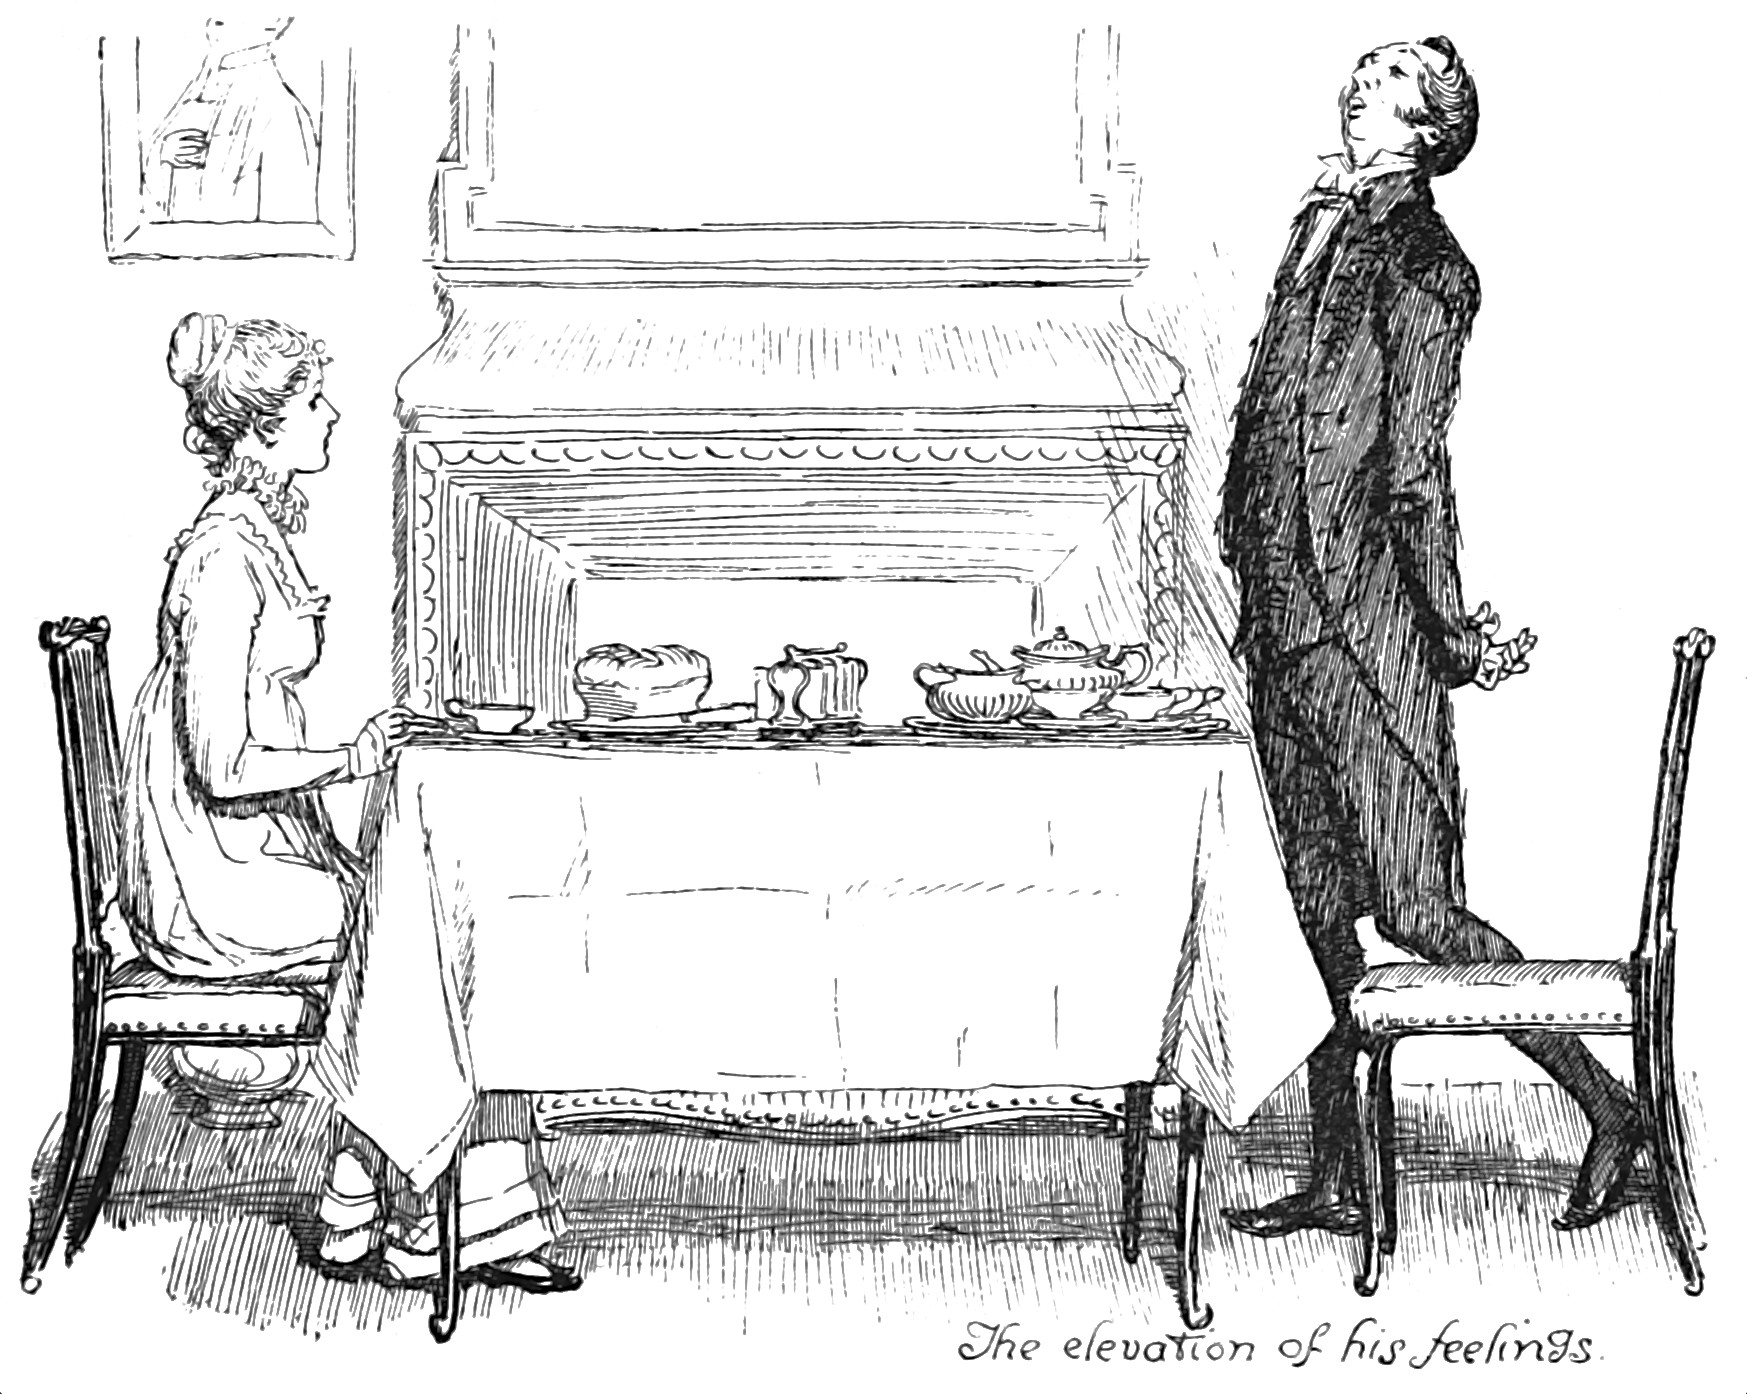
\includegraphics[width=\linewidth]{38top}
\captionlistentry{The elevation of his feelings}
\end{figure}


\lettrine[lines=6,image=true]{initials/chap38o}{n} Saturday morning Elizabeth and Mr Collins met for breakfast a few minutes before the others appeared; and he took the opportunity of paying the parting civilities which he deemed indispensably necessary.

\zz
<I know not, Miss Elizabeth,> said he, <whether Mrs Collins has yet expressed her sense of your kindness in coming to us; but I am very certain you will not leave the house without receiving her thanks for it. The favour of your company has been much felt, I assure you. We know how little there is to tempt anyone to our humble abode. Our plain manner of living, our small rooms, and few domestics, and the little we see of the world, must make Hunsford extremely dull to a young lady like yourself; but I hope you will believe us grateful for the condescension, and that we have done everything in our power to prevent you spending your time unpleasantly.>

Elizabeth was eager with her thanks and assurances of happiness. She had spent six weeks with great enjoyment; and the pleasure of being with Charlotte, and the kind attention she had received, must make \textit{her} feel the obliged. Mr Collins was gratified; and with a more smiling solemnity replied,—

<It gives me the greatest pleasure to hear that you have passed your time not disagreeably. We have certainly done our best; and most fortunately having it in our power to introduce you to very superior society, and from our connection with Rosings, the frequent means of varying the humble home scene, I think we may flatter ourselves that your Hunsford visit cannot have been entirely irksome. Our situation with regard to Lady Catherine's family is, indeed, the sort of extraordinary advantage and blessing which few can boast. You see on what a footing we are. You see how continually we are engaged there. In truth, I must acknowledge, that, with all the disadvantages of this humble parsonage, I should not think anyone abiding in it an object of compassion, while they are sharers of our intimacy at Rosings.>

Words were insufficient for the elevation of his feelings; and he was obliged to walk about the room, while Elizabeth tried to unite civility and truth in a few short sentences.

<You may, in fact, carry a very favourable report of us into Hertfordshire, my dear cousin. I flatter myself, at least, that you will be able to do so. Lady Catherine's great attentions to Mrs Collins you have been a daily witness of; and altogether I trust it does not appear that your friend has drawn an unfortunate—but on this point it will be as well to be silent. Only let me assure you, my dear Miss Elizabeth, that I can from my heart most cordially wish you equal felicity in marriage. My dear Charlotte and I have but one mind and one way of thinking. There is in everything a most remarkable resemblance of character and ideas between us. We seem to have been designed for each other.>

Elizabeth could safely say that it was a great happiness where that was the case, and with equal sincerity could add, that she firmly believed and rejoiced in his domestic comforts. She was not sorry, however, to have the recital of them interrupted by the entrance of the lady from whom they sprang. Poor Charlotte! it was melancholy to leave her to such society! But she had chosen it with her eyes open; and though evidently regretting that her visitors were to go, she did not seem to ask for compassion. Her home and her housekeeping, her parish and her poultry, and all their dependent concerns, had not yet lost their charms.

At length the chaise arrived, the trunks were fastened on, the parcels placed within, and it was pronounced to be ready. After an affectionate parting between the friends, Elizabeth was attended to the carriage by Mr Collins; and as they walked down the garden, he was commissioning her with his best respects to all her family, not forgetting his thanks for the kindness he had received at Longbourn in the winter, and his compliments to Mr and Mrs Gardiner, though unknown. He then handed her in, Maria followed, and the door was on the point of being closed, when he suddenly reminded them, with some consternation, that they had hitherto forgotten to leave any message for the ladies of Rosings.

<But,> he added, <you will of course wish to have your humble respects delivered to them, with your grateful thanks for their kindness to you while you have been here.>

Elizabeth made no objection: the door was then allowed to be shut, and the carriage drove off.

<Good gracious!> cried Maria, after a few minutes' silence, <it seems but a day or two since we first came! and yet how many things have happened!>

<A great many indeed,> said her companion, with a sigh.

<We have dined nine times at Rosings, besides drinking tea there twice! How much I shall have to tell!>

Elizabeth privately added, <And how much I shall have to conceal!>

Their journey was performed without much conversation, or any alarm; and within four hours of their leaving Hunsford they reached Mr Gardiner's house, where they were to remain a few days.

Jane looked well, and Elizabeth had little opportunity of studying her spirits, amidst the various engagements which the kindness of her aunt had reserved for them. But Jane was to go home with her, and at Longbourn there would be leisure enough for observation.

It was not without an effort, meanwhile, that she could wait even for Longbourn, before she told her sister of Mr Darcy's proposals. To know that she had the power of revealing what would so exceedingly astonish Jane, and must, at the same time, so highly gratify whatever of her own vanity she had not yet been able to reason away, was such a temptation to openness as nothing could have conquered, but the state of indecision in which she remained as to the extent of what she should communicate, and her fear, if she once entered on the subject, of being hurried into repeating something of Bingley, which might only grieve her sister further.